%\def\year{2015}
%%File: formatting-instruction.tex
%\documentclass[letterpaper]{article}
%\usepackage{aaai}
%\usepackage{amsmath,amssymb}
%\usepackage{amsthm}
%\usepackage{times}
%\usepackage{helvet}
%\usepackage{courier}
%\usepackage{graphicx}
%\frenchspacing
%\setlength{\pdfpagewidth}{8.5in}
%\setlength{\pdfpageheight}{11in}
%\pdfinfo{
%/Title (Flexibility Revisited)
%/Author (Simon Mountakis, Tomas Klos, Cees Witteveen)
%/Keywords Scheduling, Simple Temporal Networks, Flexibility}
%\setcounter{secnumdepth}{0}  
%\providecommand{\myceil}[1]{\left \lceil #1 \right \rceil }
%\providecommand{\myfloor}[1]{\left \lfloor #1 \right \rfloor }
%\newtheorem{theorem}{Theorem}
%\newtheorem{observation}{Observation}
%\newtheorem{proposition}{Proposition}
%%\newtheorem{corollary}{Corollary}
%\newtheorem{definition}{Definition}
%\newtheorem{example}{Example}
%%\newtheorem{observation}{Observation}
%%\newtheorem{remark}{Remark}
%\newcommand{\est}{\ensuremath{\mathit{est}}}
%\newcommand{\lst}{\ensuremath{\mathit{lst}}}
%\newcommand{\flex}{\ensuremath{\mathit{flex}}}
%\newcommand{\vA}{\ensuremath{\vec{A}}}
%\newcommand{\vx}{\ensuremath{\vec{x}}}
%\newcommand{\vb}{\ensuremath{\vec{b}}}
%\newcommand{\vc}[1]{\ensuremath{\vec{#1}}}
%\renewcommand{\vec}[1]{\mathbf{#1}}
%\newcommand{\BBox}{\rule{5pt}{6pt}}
%\newcommand{\blbox}{ \hfill \BBox}
%\setlength\abovedisplayskip{4pt plus 2pt minus 2pt}
%\setlength\belowdisplayskip{4pt plus 2pt minus 2pt}
%\frenchspacing
%
%%\usepackage{tikz}
%%%\usetikzlibrary{external}
%%\usetikzlibrary{arrows,automata}
%%\usepackage{subfig}
%%\usepackage{booktabs}
%%\usepackage{enumerate}
%
%\begin{document}
%
%\title{Temporal Flexibility Revisited:\\
%         \large{Maximizing Flexibility By Computing Bipartite Matchings}}
%\author{Tracking number 48}
%\author{Simon Mountakis \and Tomas Klos \and Cees Witteveen\\
%Algorithmics group, Department of Computer and Software Technology,\\
%Delft University of Technology, NL-2628 CD,
%Delft, The Netherlands\\
%}
%
%% The file aaai.sty is the style file for AAAI Press 
%% proceedings, working notes, and technical reports.
%%
%
%\maketitle
%\begin{abstract}
%
%\begin{quote}
%We discuss two flexibility metrics for Simple Temporal Networks (STNs): the so-called naive flexibility metric based on the difference between earliest and latest starting times of temporal variables, and a recently proposed concurrent flexibility metric. 
%%After an analysis based on a geometric interpretation of both metrics, we discuss an alternative method to compute these flexibility metrics. 
%We establish an interesting connection between the computation of these flexibility metrics and properties of the minimal distance matrix $D_S$ of an STN $S$:  the concurrent flexibility metric can be computed by finding a \emph{minimum} weight matching of a weighted bipartite graph completely specified by $D_S$, while the naive flexibility metric corresponds to computing a \emph{maximum} weight matching in the same graph.
%From a practical point of view this correspondence offers an advantage: instead of using an $O(n^5)$ LP-based approach, 
%%to compute the concurrent flexibility metric whose worst-case complexity is bounded by $O(n^5)$, 
%%
%reducing the problem to a matching problem we derive an $O(n^3)$ algorithm for computing the concurrent flexibility metric.
%\end{quote}
%\end{abstract}
%
\section{Introduction}
Simple Temporal Networks (STNs) \cite{dechter1991,dechter:2003}, offer a convenient framework for modelling temporal aspects of scheduling problems, distinguishing between a set $T$ of temporal variables and a set $C$ of linear difference constraints between them. STNs have been used quite extensively in a number of different domains where automated planning and scheduling are key issues, such as manufacturing, maintenance, unmanned spacecraft and robotics. One of the attractive properties of STNs is that various important search and decision problems can be solved quite efficiently. For example, deciding whether an STN admits a schedule, finding such a schedule, as well as finding a complete schedule extending a partial one are all problems that can be solved in low-polynomial time.

Constructing one single schedule, however, for an STN is often not sufficient. In quite some applications one has to react immediately to possible disturbances without having the time to recompute a new schedule. In such a case, instead of one single schedule, we would like to have a \emph{set of schedules} available from which we can select in constant time a suitable alternative. The availability of such a set of alternative schedules implies that the scheduler could offer some amount of \emph{flexibility} in scheduling: instead of determining a fixed value for a temporal variable, a flexible schedule offers for each temporal variable a set of values  to choose from.
Clearly, such a flexibility is determined by properties of the set $C$ of constraints of an STN. Therefore, one would like to specify a \emph{flexibility metric} for STNs based on the properties of this set $C$. 
One of the first proposals \cite{policella:2004,pollack:2005} for such a flexibility  metric has been based on considering a (non-empty) interval $[\est(t), \lst(t)]$ for each temporal  variable $t \in T$ and defining the flexibility of an STN $S$ as $\flex(S) = \Sigma_{t \in T} (\lst(t) - \est(t))$. Here, $\est(t)$ refers to the earliest time $t$ can be executed in any feasible schedule for $S$ and $\lst(t)$ to its latest time.
%One of the first ideas for such a flexibility has been based on the \emph{decomposability}  \cite{dechter1991,dechter:2003} of STNs. Here, decomposability refers to the property of a scheduling system that for every partial schedule that satisfies the scheduling constraints, there is always a total schedule extending it that will satisfy all the constraints.  In particular, it implies that if for a certain event $e$ there is an interval $I_e$ of time points $v_e$ that can be chosen as possible starting times for $e$, we are sure to be able to extend the partial schedule $\sigma(e)=v_e$ to a total schedule. 
%Since this idea can be used starting from any event $e$, some authors suggested to use these intervals $I_e$ of time points to achieve a flexible schedule for such a system. 
We will discuss this idea in more detail below.

As has been pointed out recently, this so-called \emph{naive flexibility metric} $\flex$ has some serious shortcomings. Its main disadvantage is that, in general, it is far too optimistic with respect to the available flexibility in an STN. The reason is that the flexibility intervals $[\est(t), \lst(t)]$ assigned to temporal variables $t$, in general, are not independent: The flexibility of two temporal variables together might be substantially smaller than the sum of their individual flexibilities \cite{wilson:2013,wilson:2014}.  As an alternative, these authors proposed to assign flexibility intervals to temporal variables such that these intervals are \emph{independent}: for every $t \in T$,  its flexibility interval $[t^-, t^+]$ enables one to make a choice for a time point in the interval without any consequence for the validity of the choices for other temporal variables. 
In their paper they use a Linear Programming (LP) based approach to compute this so-called \emph{concurrent flexibility metric} $\flex^*$ to show that it can be computed in polynomial time. They do not, however, mention exact upper bounds for the time complexity of computing this metric.

In this chapter, we start by presenting a geometric interpretation of the concurrent and the naive flexibility metric. Then, by using duality theory, we show that there exists a nice correspondence between (a slightly modified) minimal distance matrix $D_S$ associated with an STN $S$ and both flexibility metrics. If this matrix $D_S$ is conceived as the specification of weights on the edges of a (complete) weighted bipartite graph $G_S$, then the value of the concurrent flexibility metric equals the costs of a minimum matching in $G_S$, while the naive flexibility metric corresponds to the costs of a maximum matching in $G_S$.  
Using this correspondence, we are able to deduce an efficient $O(n^3)$ algorithm for determining both the concurrent and naive flexibility of an STN.

%Hier eventueel nog meer resultaten aan toevoegen.
\section{Preliminaries}
An STN  is a pair $S = (T,C)$, where $T = \{t_{0},t_{1}, \ldots, t_{n-1}\}$ is a set of temporal variables and $C$ is a finite set of binary constraints on $T$, each constraint having the form\footnote{If both $t_{j}-t_{i}\leq c_{ij}$ and $t_{i}-t_{j}\leq c_{ji}$ are specified, we will also use the more compact notation $- c_{ji}\leq t_j - t_i \leq c_{ij}$ 
%or $t_j - t_i  \in [-c_{ji},c_{ij}]$
.} 
$t_{j}-t_{i}\leq c_{ij}$, for some real number $c_{ij}$. 
A solution to $S$ is a \emph{schedule} for $S$, that is, a function $\sigma: T \rightarrow \mathbb{R}$, assigning a real value (time-point) to each temporal variable in $T$ such that all constraints in $C$ are satisfied. If such a schedule exists, we say that the STN is \emph{consistent}.\footnote{Without loss of generality, in the remainder of the paper, we assume that an STN to be consistent. Note that consistency of an STN can be determined in low-order polynomial time~\cite{dechter1991}.}
The time-point $t_{0} \in T$, also denoted by $z$, is used to be able to express absolute time constraints. It represents a fixed reference point on the timeline, and is assigned the value $0$. 
%Often we represent an STN $S = (T, C)$ as a directed weighted graph $G_S = ( T_S, E_S, l_S )$ where the vertices $T_S$ represent variables in $T$ and for every constraint $t_j - t_i \leq c_{ij}$ in $C$ there is a directed edge $(t_i, t_j) \in E_S$ labeled by its weight $l_S(t_i, t_j) = c_{ij}$. In this paper, we will use both representations interchangeably and will not make a distinction between the nodes in $T_S$ and variables in $T$, nor between the constraints in $C$ and the labeled edges in $E_S$.
\begin{example} \label{ex.1}
We consider two STNs $S_1 = (T_1, C_1)$ and $S_2 = (T_2, C_2)$ where $T_1 = T_2 =  \{z, t_1, t_2, t_3\}$ and
\begin{align*}
C_1 = \quad&\{ 0 \leq t_i - z \leq 50 \mid i=1,2,3 \}, \\
C_2 = \quad&C_1 \; \cup 
%C_2 = \quad&\{ 0 \leq t_i - z \leq 50 \mid i=1,2,3 \} \; \cup \\
 \; \{ 0 \leq t_i - t_j \leq \infty \mid 1 \leq j < i \leq 3 \}.
\end{align*}
 Every assignment $\sigma_1(t_i) = v_i\in [0,50]$ is a schedule for $S_1$.  On the other hand, a schedule $\sigma_2$ for $S_2$ has to satisfy $0 \leq \sigma_2(t_1) \leq \sigma_2(t_2) \leq \sigma_2(t_3) \leq 50$. 
\end{example}
%The graph representation is very helpful in finding tighter constraints implied by the set $C$ of constraints, interpreting the weights $c_{ij}$ on the arcs as lengths of the path from $t_i$ to $t_j$. 
%\footnote{For example, since $C_2$ contains the constraints $t_2 - t_0 \leq 50$ and $t_0 - t_1\leq 0$, then there exists a path from $t_2$ via $t_0$ to $t_1$ having a length $50+0 =50$. This makes 
%$ t_2 -t_1 \leq 50 $ an \emph{implied} constraint that is tighter than the given constraint $t_2 - t_1 \leq \infty$.}
Using a shortest path interpretation of an STN $S=(T,C)$ \cite{dechter:2003}, there is an efficient method to find all tightest constraints implied by $C$, by searching for all shortest paths between the time points in $T$ using e.g.\ Floyd and Warshall's all-pairs shortest paths algorithm \cite{floyd:1962}. The $n\times n$ \emph{minimum distance matrix} $D_S$ contains for every pair of time-point variables $t_i$ and $t_j$ the length $D_S[i,j]$ of the \emph{shortest path} from $t_i$ to $t_j$ in the distance graph. In  particular, 
%the first row and the first column of the distance matrix $D_S$ contain useful information about the possible schedules for $S$.
%Note that the first row of $D_S$ contains all entries $D_S[0,i]$ such that $t_i - z = t_i \leq D_S[0,i]$. This means that any schedule for $S$ should satisfy $t_i \leq D_S[0,i]$. Hence, $D_S[0,i]$ is $t_i$'s \emph{latest starting time}, denoted by $\lst(t_i)$ and the assignment $\sigma_{\max}(t) = \lst(t)$, $\forall t \in T$, is the maximum schedule for $S$.
the latest starting time $\lst(t_i)$ and earliest starting time $\est(t_i)$ can be obtained directly from the first row and first column of $D_S$: $\lst(t_i) = D[0,i]$ and $\est(t_i) = -D[i,0]$.
% $t_i$'s \emph{latest starting time}, denoted by $\lst(t_i)$ and the assignment $\sigma_{\max}(t) = \lst(t)$, $\forall t \in T$, is the maximum schedule for $S$.
%Analogously, the first column of the distance matrix contains entries $D_S[j,0]$ such that $z - t_j \leq D_S[j,0]$, i.e.,
%$t_j -z = t_j\geq -D_S[j,0]$.  So $-D_S[j,0]$ is $t_j$'s \emph{earliest starting time}, denoted by $\est(t_j)$. The assignment $\sigma_{\min}(t) = \est(t)$, $\forall t \in T$, is the minimum schedule for $S$.
Given an STN $S$, this matrix $D_S$ can be computed in low-order polynomial ($O(n^3)$) time  \cite{dechter:2003}. Here, $n$ denotes the number of temporal variables.
%\footnote{A recent improvement by Planken et al.~\cite{planken:2012} has shown that a schedule can be found in $O(n^2w_d)$-time where $w_d$ is the graph width induced by a vertex ordering.} 

The following proposition is a restatement of Theorem~3.3 in \cite{dechter1991} and essentially states that every STN is decomposable via its distance graph $D_S$:
\begin{proposition}\label{estlst}
Let $S = (T, C)$ be an STN and $D_S$ its distance matrix. For $i=1, \ldots, n-1$, let $\est(t_i) = -D_S[i,0]$ and $\lst(t_i) = D_S[0,i]$.
Then, for every schedule $\sigma$ for $S$, and every $t \in T$, it holds that $\sigma(t) \in [\est(t), \lst(t)]$.
Moreover, given any $t \in T$ and $v \in [\est(t), \lst(t)]$, there exists a schedule $\sigma$ for $S$ such that $\sigma(t) = v$.\footnote{In fact it can be shown that there exists a simple backtrack-free polynomial-time algorithm to construct such a schedule $\sigma$ for $S$.}
\end{proposition}
Finally, we assume that for each $t \in T$ there is a finite interval for scheduling it. In particular this means that for each STN $S = (T, C)$ we assume that for all $t \in T$, $t \geq z$ holds and there exists a finite constant (horizon) $h_{S}$ such that for all $t \in T$ it holds that $t \leq h_{S}$. This avoids the use of unbounded time intervals such as $-\infty \leq t_i - t_j \leq \infty$.

\section{The naive and the concurrent flexibility metric}

Intuitively, a flexibility metric should indicate our freedom of choice in choosing values for temporal variables such that  the constraints are satisfied. In the naive flexibility metric one has chosen, for each variable $t \in T$, the interval $[\est(t), lst(t)]$ to indicate this freedom of choice.\footnote{One of the reasons for this choice is that taking any value $v \in [\est(t), lst(t)]$ for $t$ allows us, by decomposability (Proposition~\ref{estlst}), to extend the partial schedule $\sigma(t)=v$ to a total schedule $\sigma$ for an STN $S$.}
The naive flexibility of an STN $S$ then is defined as $\flex(S) = \sum_{t \in T}\; (\lst(t) - \est(t))$. 
Obviously, since $D_S$ is computable in $O(n^3)$ time, $\flex(S)$ can be computed in $O(n^3)$ time. 

As we already mentioned, using $\flex(S)$ has a serious disadvantage, due to \emph{dependencies} that might exist between temporal variables. We give a simple example to illustrate these dependencies and their consequences.
\begin{example}
Consider the STNs presented in Example~\ref{ex.1}.
For both STNs it holds that $\est(t_i) = 0$ and $\lst(t_i) = 50$, for $i=1,2,3$.
Hence, $\flex(S_1)= \flex(S_2) = 150$.
Intuitively, however, due to the ordering constraints between $t_1$, $t_2$ and $t_3$, the flexibility of $S_2$ should be much lower: giving a flexibility of $f_1$ to $t_1$ results in a flexibility of $f_2 = v_2 - f_1$  for $t_2$, where $50 \geq v_2 \geq f_1$, and a flexibility of $50 - v_2$ for $f_3$. The sum of these flexibilities equals $f_1+(v_2 - f_1) + (50 - v_2) = 50$, one-third of the value of the naive flexibility for $S_2$.
\end{example}
 %One way to see how these dependencies are neglected in computing the naive flexibility $\flex(S)$ is to frame the computation of $\flex(S)$ as a linear program. To this end, consider the following LP:
%\begin{alignat*}{2}  \label{LP1} \tag{LP1}
%\text{maximize}   &\quad \sum_{t \in T}{(t^+ - t^-)}\ \\
%\text{subject to } 
%                         &\quad t^+_j - t^+_i     \leq  c_{i,j}  &, & \quad \forall\;( t_j - t_i \leq c_{i,j}) \in C   \\ 
%                         &\quad t^-_j - t^-_i       \leq  c_{i,j}  &, & \quad \forall\;( t_j - t_i \leq c_{i,j}) \in C
%                        \end{alignat*}
%It is easy to see that $\flex(S)$ is the maximizer of this linear program.
%First of all, $\flex(S)$ is an upper bound for $\sum_{t \in T}{(t^+ - t^-)}$, since 
%$ \max \sum_{t_i \in T}{(t_i^+ - t_i^-)} \leq  \max \{ \sum_{t_i \in T} t_i^+ \}- \min \{ \sum_{t_i \in T} t_i^- \}  \leq  \sum_{t_i \in T} \lst(t_i) - \sum_{t_i \in T} \est(t_i) 
%     = \flex(S).$ 
%% \begin{align}
%% \max \sum_{t_i \in T}{(t_i^+ - t_i^-)} \leq &\quad \max \{ \sum_{t_i \in T} t_i^+ \}- \min \{ \sum_{t_i \in T} t_i^- \} \notag\\
%%    \leq &\quad \sum_{t_i \in T} \lst(t_i) - \sum_{t_i \in T} \est(t_i) \notag \\
%%     = &\quad \flex(S) \notag
%% \end{align}
% On the other hand, since $S$ is an STN, the assignment $\sigma$ such that  for $i=1,\ldots, n$, $\sigma(t^+_i) = \lst(t_i)$ and $\sigma(t^-_i) = \est(t_i)$, 
%is a feasible  solution of \ref{LP1}.
%Hence, $ \flex(S) \leq \max \sum_{t_i \in T}{(t_i^+ - t_i^-)}$.
%% \begin{align}  
%%  \sum_{t_i \in T}{(lst(t_i) - est(t_i) ) = \flex(S)} \leq \max \sum_{t_i \in T}{(t_i^+ - t_i^-)} \notag
%% \end{align}
% % Therefore, $\flex(S) \leq \max \sum_{t_i \in T}{(t_i^+ - t_i^-)}$.
% 
%The solution space of a linear program such as \ref{LP1} is a polytope. In case of a consistent STN it is a bounded polytope. The maximizer of \ref{LP1} can be thought of as determining the smallest (hyper)cube containing the polytope generated by the underlying STN. Clearly, if the polytope generated by an STN $S$ is not a hypercube, there are points in the hypercube which do not belong to the solution space of the STN. Exactly in these cases $\flex(S)$ will overestimate the amount of flexibility of $S$. 

One way to see how these dependencies are neglected in computing the naive flexibility $\flex(S)$ is to give a geometric interpretation of this metric.  
 
The solution space of a set of linear constraints is a polytope. In (our) case of a consistent STN it is a bounded polytope. The set of intervals $\{ [\est{(t_i)},\lst{(t_i})]\}^n_{i=1}$ can be thought of as determining the smallest (hyper)cube containing this polytope. Clearly, if the polytope itself is not a hypercube, there are points in the hypercube that do not belong to the solution space of the STN. Exactly in these cases $\flex(S)$ will overestimate the amount of flexibility of $S$. 
\begin{example}
Consider again the STNs $S_1$ and $S_2$ as presented in Example~\ref{ex.1}. 
The polytope generated by $C_1$ is the large (hyper)cube depicted in Figure~\ref{Fig1}. This hypercube equals the smallest hypercube containing the polytope, hence $\flex(S_1)= 50 + 50+50$ is the real flexibility of $S_1$.
The polytope generated by $C_2$ is the shaded subspace depicted in Figure~\ref{Fig1}. The smallest hypercube containing it, however, equals the hypercube specified for $S_1$. Hence, $\flex(S_2)= \flex(S_1) =150$: an overestimation of the flexibility.

\begin{figure}
\centering
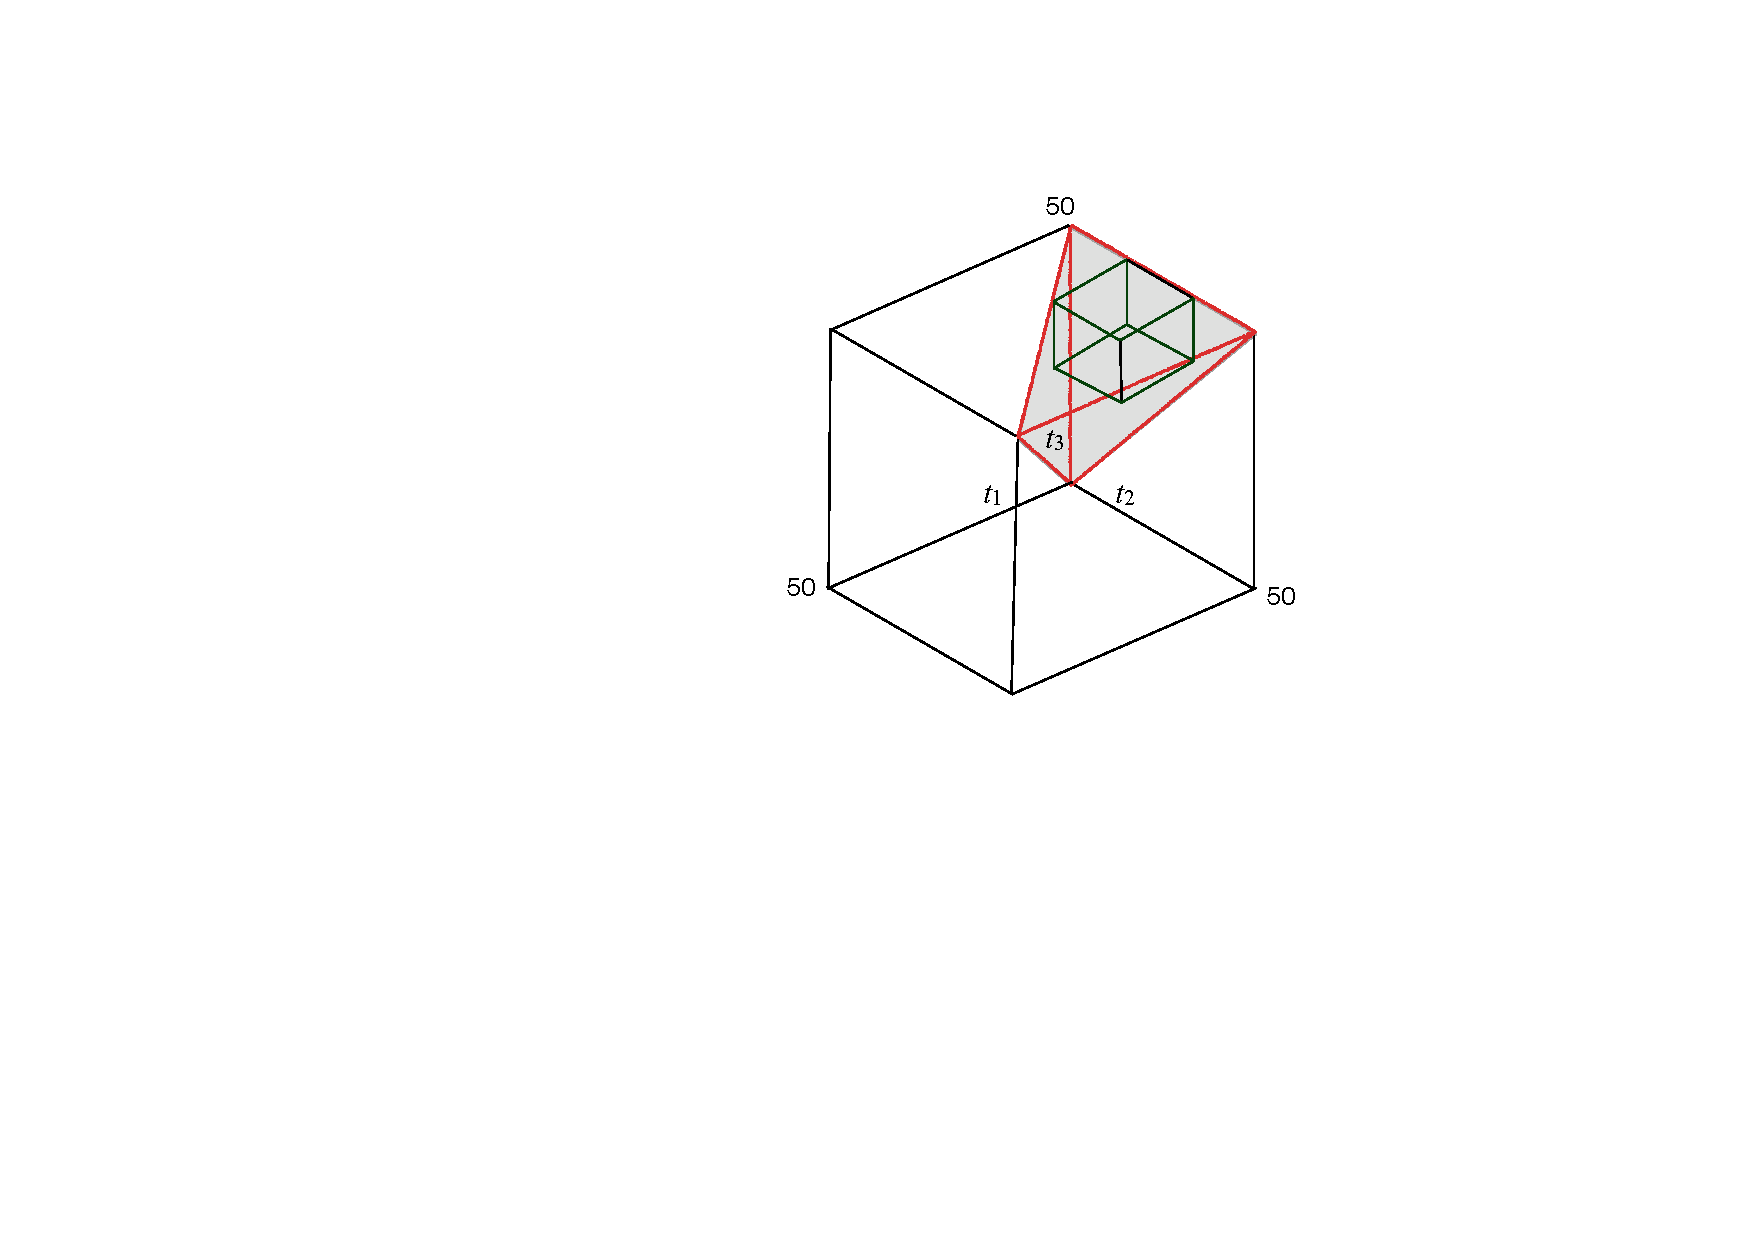
\includegraphics[width=0.3\textwidth]{chapter/icaps-flexibility/polytopes.pdf}
\caption{The polytope $P_1$ generated by $S_1$ is a cube with edges of size 50; the polytope $P_2$ generated by $S_2$ is the shaded subspace of $P_1$. The inner bounding box of $P_2$ is the small green cube in the shaded area. The inner bounding box of $S_1$ and also the outer bounding box of $S_1$ and $S_2$ equal $P_1$.}
\label{Fig1}
\end{figure}
\vspace{-0.8cm}\mbox{}\\
\end{example}
A new flexibility metric for STNs  \cite{wilson:2013} has been introduced to overcome the disadvantages of $\flex(S)$.
Instead of determining the smallest \emph{outer bounding box} (hypercube) containing the polyhedron generated by a set of constraints $C$, they determine the largest \emph{inner bounding box} contained in this polyhedron (see below for a computation).
An obvious advantage of such an inner bounding box is that every point in the box belongs to the polyhedron (i.e.\ solution space) containing it.
\begin{example}
Consider again the STN $S_2$. A largest inner bounding box contained in the polytope determined by $C_2$ is the small box contained in the shaded area in Figure~\ref{Fig1}. All its points are contained in the solution space of $S_2$.
\end{example} 
To construct a flexibility metric based on the largest inner bounding box we have to make sure that for every constraint $t_j - t_i \leq c_{i,j}$  the flexibility intervals  $[t^-_i, t^+_i]$ and $[t^-_j, t^+_j]$ associated with $t_i$ and $t_j$ are independent, i.e., every value $v_i$ and $v_j$ for $t_i$ and $t_j$, respectively, chosen in these intervals has to satisfy the constraint $v_j - v_i \leq c_{i,j}$. 
This is exactly the case if $t_j$ assumes the maximum value and $t_i$ assumes the minimum value in its interval, i.e., we have to ensure that $t^+_j - t^-_i \leq c_{i,j}$.
Therefore, the value $\flex^*(S)$ for the concurrent flexibility for $S$ can be found by solving the following LP (see \cite{wilson:2014}):
%The key idea in using the largest inner bounding box is that a flexibility metric based on it ensures that all dependencies between the flexibility intervals $[t^-_i, t^+_i]$ have been removed.
%In order to guarantee complete independence between these intervals, we have to make sure that the upper bounds and lower bounds of these intervals satisfy the constraints imposed on them.
%For example, consider aBut that is the case exactly if $t_j$ is maximal and $t_i$ is minimal, i.e., we have to ensure that $t^+_j - t^-_i \leq c_{i,j}$.
%As we have developed our arguments in detail elsewhere~\cite{wilson:2014-aij}, in this paper we will only give the solution we propose. It consists of assigning an interval to each variable from which \emph{every} value can be chosen, \emph{independently} from the values chosen for other variables. We call such an assignment an \emph{interval schedule}. An STN's flexibility, denoted by $\flex(S)$, will measure the sum of the lengths of these intervals.
%
%\begin{definition}[Interval schedule]
%Given an STN $S=(T,P)$, a set $I_S=\{I_t=[\ell_t,u_t]\mid t\in T\}$ of non-empty intervals for the time point variables $t\in T$ is an \emph{interval schedule} for $S$ iff for every $t\in T$ and every $v_t\in[\ell_t,u_t]$, the assignment $\sigma$ defined by $\sigma(t)=v_t$ is a schedule for $S$.
%\end{definition}
%
%To compute an interval schedule, we transform the STN $S$ to an STN $S'$ in which new variables $t^-_i$ and $t^+_i$ occur for every $t_i\in T$. These variables model the lower and upper boundaries of the interval assigned to variable $t_i$.
%In order to ensure that the variables $t^-_i$ and $t^+_i$ correspond to their intended meaning, we need to make sure that for every constraint $t_j - t_i\leq c_{i,j}$ in $P$, the intervals assigned to these events should be constrained so that, within their respective intervals, the events can not be scheduled so far apart as to violate the constraint.
%
%\begin{proposition}\label{prop:independent}
%Let $S = (T,P)$ be an STN. A set $I_S = \{ [\ell_{t}, u_{t}]\mid t \in T\}$ of intervals for the variables in $T$ is an interval schedule for $S$, iff for every pair $(t_i, t_j) \in T^2$, %niet T \cup \{z\}, want z zit al in T
%it holds that if $t_j - t_i \leq c_{ij} \in P$, then $u_{t_j} - \ell_{t_i} \leq c_{ij}$.
%\end{proposition}
%\begin{proof}
%(If) Suppose the implication holds for every pair of variables. We have to show that $I_S$ is an interval schedule. So, for every $t \in T$, choose an arbitrary value $v_t \in [ \ell_{t}, u_{t}]$ and let $\sigma$ be defined by $\sigma(t)=v_t$, for all $t\in T$. We must show that $\sigma$ is a schedule for $S$. Suppose $\sigma$ is not a schedule, but that it violates some constraint in $P$, say $t_j - t_i \leq c_{ij}$. Observe that we have assumed that the fact that this constraint is an element of $P$, implies that $u_{t_j} - \ell_{t_i} \leq c_{ij}$. The fact that this constraint is violated by $\sigma$ means that $\sigma(t_j) - \sigma(t_i) > c_{ij}$. But this implies that $c_{ij} < v_{t_j} - v_{t_i} \leq u_{t_j} - \ell_{t_i}$, since $v_{t_j}\leq u_{t_j}$ and $v_{t_i}\geq\ell_{t_i}$. Thus $u_{t_j} - \ell_{t_i}>c_{ij}$, which contradicts the fact that $u_{t_j} - \ell_{t_j} \leq c_{ij}$, so $\sigma$ is a schedule for $S$.
%
%(Only if) Suppose the set $I_S$ is an interval schedule for $S$. Take an arbitrary pair $(t_i,t_j)\in T^2$, and suppose $t_j-t_i\leq c_{ij}\in P$. Because $I_S$ is an interval schedule, there is a schedule $\sigma$ for $S$ such that $\sigma(t_j)=u_{t_j}$ and $\sigma(t_i)=\ell_{t_i}$. Because $\sigma$ is indeed a schedule, it satisfies all constraints in $P$, so we know that $u_{t_j}-\ell_{t_i}\leq c_{ij}$. 
%\end{proof}
%
%This result tells us which constraints the endpoints of an interval schedule have to satisfy. We will therefore view the interval \emph{endpoints as variables}, and compute values for them when they are subjected to these constraints. In particular, from the STN $S$ we compute interval endpoints as the solution of a derived STN $S'=(T',P')$, which has two interval end points $t_i^-$ and $t_i^+$ for every $t_i\in T$. We have just seen intuitively how we should fill the set of constraints $P'$. More precisely, to $P'$ we add a constraint $t_j^+-t_i^-\leq c_{ij}$  for every constraint $t_j-t_i\leq c_{ij}$ in $P$, and a constraint $t_i^--t_i^+\leq 0$ for every $t_i\in T$.
%
%\begin{proposition}
%Let $S =(T,P)$ be an STN. Consider the STN  $S' = (T', P')$ where
%\begin{align*}
%T' = &\ \{ t^+, t^- \mid t \in T \} \cup \{z'\}, \\
%P' = &\ \{ t^+ - t'^- \leq c \mid t - t' \leq c \in C \}\ \cup \\
%&\ \{ t^- -t^+ \leq 0 \mid t\in T \}\ \cup\\
%&\ \{ z' - t_0^- \leq 0, t_0^+-z'\leq0\}.
%\end{align*}
%Then, for every solution $\sigma'$ of $S'$, the set $\{ [\sigma'(t^-), \sigma'(t^+)] \mid t \in T \}$ is an interval schedule for $S$.
%\end{proposition}
%\begin{proof}
%First we establish that there actually exists a solution $\sigma'$ for $S'$. We have assumed that $S$ is consistent, so there exists a schedule $\sigma$ for $S$. Take such a schedule, and construct an assignment $\sigma'$ for $S'$ as follows: For every $t\in T$, let $\sigma'(t^+)=\sigma'(t^-)=\sigma(t)$. It can readily be verified from the construction of the set $P'$ that $\sigma'$ satisfies all those constraints.
%
%So we can now take an arbitrary schedule $\sigma'$ for $S'$ and show that the set $\{[\sigma'(t^-),\sigma'(t^+)]\mid t\in T\}$ is an interval schedule for $S$. Take an arbitrary constraint $t_j-t_i\leq c_{ij}\in P$. By Proposition~\ref{prop:independent} it suffices to show that $\sigma'(t_j^+)-\sigma(t_i^-)\leq c_{ij}$. Because the constraint $t_j-t_i\leq c_{ij}\in P$, the constraint $t^+_j-t^-_i \leq c_{ij}$ was added in the construction of $P'$, and since $\sigma'$ is a schedule for $S'$, it satisfies this constraint.
%\end{proof}
%
%Although our transformation of $S$ into $S'$ provides us with an interval schedule for $S$, we have yet to determine the flexibility of $S$, since the sum of the sizes of these intervals does not need to be maximal.
%To obtain the flexibility  measure, we have to select a solution $\sigma'$ for $S'$ that maximizes the sum of the sizes of the intervals.
%%To take into account these dependencies, for every $t_i \in T$  respectively. For every $t_i$ we also define a function $f_i$ that returns the interval (flexibility) $(t^-_i, t^+_i)$ for $t_i$ \emph{given} the corresponding intervals (flexibilities) $(t^-_j, t^+_j)$ for all other events $t_j \neq t_i$. In general,
%%\[
%%f_i((t^-_1, t^+_1), \ldots (t^-_{i-1}, t^+_{i-1}), (t^-_{i+1}, t^+_{i+1}), \ldots, (t^-_{n}, t^+_{n})) = (t^-_i, t^+) \]
%%
%%This function $f_i$ is specified such that 
%%\begin{enumerate}
%%\item every starting time $v \in (t^-_i, t^+)$ can be chosen for $t_i$, whatever starting times in the intervals  $(t^-_j, t^+_j)$ are chosen for the other events, 
%%\item the size $t^+_i - t^-_i$ of the interval $[ t^-_i , t^+_i ]$ is maximal.
%%\end{enumerate}
%%In other words, the flexibility $flex(t_i) = (t^+_i - t^-_i)$ is a real flexibility assigned to event $t_i$ and is independent of the flexibilities $flex(t_j) = (t^+_j - t^-_j)$ assigned to other events.
%%Since we would like to maximise the sum $\Sigma^n_{i=1} flex(t_i)$ as a metric for the real flexibility of $S$, we define $flex(S)$ as follows:
%%\begin{equation}\label{flex.1}
%% flex(S) = max_{t^-_1, t^+_1, \ldots t^-_n, t^+_n}\Sigma^n_{i=1} (t^+_i - t^-_i)
%%\end{equation}
%%where
%%\[ f_i((t^-_1, t^+_1), \ldots (t^-_{i-1}, t^+_{i-1}), (t^-_{i+1}, t^+_{i+1}), \ldots, (t^-_{n}, t^+_{n})) = (t^-_i, t^+_i) \]
%%
%%The problem to find a suitable flexibility metric now has been reduced to finding suitable functions $f_i$ satisfying the requirements mentioned.
%%Fortunately, due to the fact that possible correlations between events are specified through linear constraints in an STN, we can easily 
%%find suitable specifications for such functions $f_i$:
%%\begin{proposition}
%%Let $S = (T, C)$ be an STN. If, for $j =1, \ldots, i-1, i+1, \ldots n$ the intervals $(t^-_j, t^+_j)$ are given, the function 
%%
%%$f_i((t^-_1, t^+_1), \ldots (t^-_{i-1}, t^+_{i-1}), (t^-_{i+1}, t^+_{i+1}), \ldots, (t^-_{n}, t^+_{n})) = (t^-_i, t^+_i)$
%%
%%\noindent 
%%can be specified as follows:
%%\begin{enumerate}
%%\item
%%$t^+_i$ is the maximal value of the variable $t_i$ satisfying all constraints $t_i - t^-_j \leq c_{ij} \in C$ as well as the constraint $t_i -z \leq c_i \in C$;
%%\item
%%$t^-_i$ is the minimal value of the variable $t_i$ satisfying all constraints $t^+_j - t_i \leq c_{ij} \in C$ as well as the constraint $z -t_i \leq c'_i \in C$.
%%\end{enumerate}
%%\end{proposition}
%%
%%\begin{proof}
%%\end{proof}
%We then need the following LP to find the maximizer that will guarantee a set of maximal and independent flexibilities:

%\begin{theorem}\label{thm:maxFlex}
%Let $S = (T, P)$ be an STN. Then $\flex(S)$ can be computed by solving the following linear program:
%\marginpar{We need to motivate $t^- \leq t^+$ here and to show that this condition does not affect the optimum }
\begin{alignat*}{2}\label{LP1} \tag{LP1}
\text{maximize}                      &\quad \sum_{t_i \in T}{(t^+_i - t^-_i)}  \\
\text{subject to }  &\quad  t^-_i                         \leq t^+_i  &, & \quad \forall\; t_i\in T  \\  
                            &\quad  t^+_j - t^-_i                 \leq  c_{i,j}   &, & \quad \forall\;( t_j  - t_i  \leq c_{i,j}) \in C
\end{alignat*}
%\end{theorem} 

%As a consequence, we have the following corollary.
%\begin{corollary} \label{obs.1}
%Given an STN $S = (T,P)$,  the  flexibility metric $\flex$ determines an assignment $\flex(t) = [t^-, t^+]$, such that for every $t \in T$ and every $v_t \in [t^-, t^+]$, the assignment $\sigma(t) = v_t$ is a fixed-time schedule for $S$ (and thus satisfies all constraints in $C$).
%\end{corollary}

%\begin{example}
%%\marginpar{(Text needs to adapted)}
%If we apply this method to the example from the previous section, we find that for this STN $S$, $\flex(S)=7$, which is attained by the following interval schedule:
%\begin{align*}
%\sigma'(z^-)&=0 &\sigma'(z^+)&=0 \\
%\sigma'(e_1^-)&=0&\sigma'(e_1^+)&=1\\
%\sigma'(e_2^-)&=5&\sigma'(e_2^+)&=5\\
%\sigma'(c_1^-)&=2&\sigma'(c_1^+)&=3\\
%\sigma'(c_2^-)&=5&\sigma'(c_2^+)&=5\\
%\sigma'(b^-)&=5&\sigma'(b^+)&=10\\
%\end{align*}
%We see that the flexibility that can be attained is much lower than as computed by the other methods mentioned earlier. Of course, other schedules are possible as well, for example, where all bounds are shifted in time. %All flexibility-maximizing interval schedules have in common that one unit of flexibility is divided among the two variables $e_1$ and $e_2$, and that this is also the case for the two variables $c_1$ and $c_2$, and that five units of flexibility is assigned to the event $b$.
%\end{example}
Here, $\flex^*(S)$ indicates the maximum flexibility that can be obtained when all flexibility intervals of temporal variables are independent from each other and values in these intervals can be chosen concurrently.
\begin{example}
 \emph{\ref{LP1}} will return $\flex^*(S_1) = 150$, but $\flex^*(S_2) = 50$, showing that here the concurrent flexibility metric corresponds to our intuition.
\end{example}

\section{Concurrent flexibility by minimum matching}
In this section we show that computing the maximum concurrent flexibility is identical to computing a perfect minimum weight matching of a weighted bipartite graph $G_S$ completely specified by $D_S$. On the other hand, computing the naive flexibility corresponds to computing a maximum matching in this graph $G_S$.

To establish these results, first, we specify an LP equivalent to \ref{LP1} using the minimum distance matrix $D_S$ instead of the original set $C$ of constraints. 
Then we show that the entries of $D_S$ can be used to compute a least upper bound on $\flex^*(S)$.
Finally, by using duality theory in Linear Programming and some adaptations, we show that this least upper bound is a maximum matching in a bipartite graph specified by $D_S$ and in fact equals $\flex^*(S)$.
 
Remember that the entries $d(i,j)$ of the minimum distance matrix $D_S$ of an STN $S$ specify the upper bound of the strongest difference constraint between the temporal variables $t_j$ and $t_i$:
$t_j - t_i \leq d(i,j)$. 
%Referring to the derivation of $\flex^*(S)$ we note that in using these strongest constraints, $t_j - t_i \leq d(i,j)$ implies that $t^+_j - t^-_i \leq d(i,j)$.
Hence, we can replace the specification \ref{LP1} by the following equivalent LP, since both LP's specify the same solution space:
\begin{alignat*}{2}\label{LP2} \tag{LP2}
\text{maximize}                       &\quad \sum_{t_i \in T}{(t^+_i - t^-_i)}  \\
\text{subject to }  &\quad t^-_i                       \leq t^+_i  &\quad , &\quad \forall\; t_i \in T \notag \\
                           &\quad t^+_j - t^-_i                  \leq  d(i,j)  &\quad , &\quad \forall\; t_i \neq t_j \in T \notag
\end{alignat*}

To remove the condition $\forall\; t_i \neq t_j \in T$, it is sufficient to realize that $
t^+_i - t^-_i = (t^+_i - t^-_0) + (t^+_0 - t^-_i) 
                    \leq d(0,i)+d(i,0) = \lst(t_i) -  \est(t_i)$,
since $t^-_0 = t^+_0 = 0$.
Hence, setting $ d(i,i) = d(0,i)+d(i,0)$ for all $t_i \in T$, we change \ref{LP2} to the following equivalent LP:
\begin{alignat*}{2}\label{LP4} \tag{LP3}
\text{maximize}                       & \sum_{t_i \in T}{(t^+_i - t^-_i)} & \\
\text{subject to }  &  t^-_i                        \leq t^+_i &\quad, \quad & \forall\; t_i \in T \notag \\
                            & t^+_j - t^-_i                  \leq  d(i,j)  &\quad, \quad  & \forall\; t_i, t_j \in T \notag
\end{alignat*}

We will denote this modified distance matrix $D_S$, where $d(i,i) = \lst(t_i)-\est(t_i)$, by $D^*_S$.

Now consider the sum
$\sum^n_{i=1} (t^{+}_i - t^-_i) $
we want to maximize.
%The concurrent flexibility $\flex^*$ is computed as the maximum of this sum under the constraints as given in \ref{eq.?}.
This sum can be rewritten as
$\sum^n_{i=1} (t^{+}_i - t^-_i)  = \sum^n_{i=1} (t^+_i - t^-_{\pi(i)})
$
for an arbitrary permutation $\pi$ of $(1,2, \ldots, n)$.
Since $t^+_i -  t^-_{\pi(i)} \leq d(\pi(i),i)$, we can derive an upper bound on this sum for every permutation $\pi$:
$  \sum^n_{i=1} (t^+_i - t^-_{\pi(i)}) \leq \sum^n_{i=1} d(\pi(i),i)$.
In particular, there are permutations $\pi^*$ such that for all permutations $\pi$ it holds that
$  \sum^n_{i=1} d(\pi^*(i),i) \leq \sum^n_{i=1} d(\pi(i),i) $.
Such a (smallest) permutation $\pi^*$ specifies a least upper bound on $\flex^*(S) = \max  \sum^n_{i=1} (t^{+}_i - t^-_i)$.

There is an efficient  way to compute such a smallest permutation $\pi^*$ by obtaining a \emph{minimum weighted matching} between $T^+ = \{t^+_1, t^+_2, \ldots, t^+_n\}$ and $T^- = \{t^-_1, t^-_2, \ldots, t^-_n\}$:
Consider the weighted complete graph $G_S = (V, E, w)$ where $V = T^+ \cup T^-$, the edges $\{t^+_i, t^-_j \} \in E$ for $i, j =1,\dots n$, and for every edge $\{t^+_i, t^-_j\}$ its weight $w_{i,j} = d_{j,i}$. Note that $G_S$ is completely specified by $D^*_S$.
By Hall's theorem, this graph has a minimum weighted perfect matching, that is a set $M \subseteq E$ of $n$ edges covering $T^+$ and $T^-$ such that the sum of these edges is minimum.
Clearly,  such a minimum weighted matching determines a permutation $\pi^*$ such that  $\sum^n_{i=1} d(\pi^*(i),i)$ is minimum.
Since it holds that $ \sum_{t_i \in T}(t^+_i - t^-_i) \leq \sum^n_{i=1} d(\pi^*(i),i)$,
the cost $c(M)$ of such a minimum matching provides an upper bound for $\flex^*(S)$.

Actually, by applying simple LP-duality theory, we can do  better and show that there exists an \emph{exact} correspondence between a minimum matching in $D^*_S$ and the maximum concurrent flexibility $\flex^*(S)$:

\begin{proposition}
Let $S = (T,C)$ be a consistent STN having a minimum distance matrix $D_S$. Then the concurrent flexibility $\flex^*(S)$ of $S$ equals the cost $c(M)$ of a minimum matching $M$ of the complete weighted graph $G_S$ specified by $D^*_S$.
\end{proposition}
\begin{proof}
The most elegant way to prove this result is making use of duality in linear programming.
The dual of \ref{LP4} is the following LP:
\begin{alignat*}{2}
\label{LP5} 
\tag{LP4}
\text{minimize}                       &\quad \sum_{1 \leq i,j \leq n} d(i,j) \, y_{j,i} \\
\text{subject to }  &\quad  \sum^n_{j=1} y_{i,j} = 1  + y_{0,i} \quad                &, &\; i \in \{1,2,\ldots n\} \notag \\
                           &\quad  \sum^n_{i=1} y_{i,j}               = 1  + y_{0,j} \quad &, &\; j \in \{1,2,\ldots n\} \notag \\
                           &\quad  y_{i,j} \geq 0 \quad & , &\; i,j \in \{0,1,\ldots, n \} \notag
\end{alignat*}
Since the original LP (\ref{LP4}) has an optimal solution, by strong duality, the objective values of optimal solutions of both LP's coincide. 
The constraint matrix associated with both LP's is total unimodular, hence, \ref{LP5} has integral optimal solutions.
This dual \ref{LP5} can be interpreted as follows: 
%assume all $y_{0,i} = 0$ for all $i=1,2, \ldots n$ and 
Let $G_S$ be a complete bipartite graph having two sets of nodes  $A = \{1, \ldots, n \}$ and $B = \{1, \ldots n \}$, representing the rows and columns of $D^*_S$. Let $D^*_S$ specify the weights $d(j,i)$ of the edges $e=(i,j)$ of $G_S$.
Then, in case $y_{0,i} = 0$ for all $i=1,2, \ldots n$), it is not difficult to see that a minimizer for \ref{LP5} specifies a minimum weight matching $M$ in $G_S$.
By strong duality, the cost $c(M)$ of $M$ corresponds to  $\flex^*(S)$.
 
Therefore, the only part left to prove is to show that the assumption $y_{0,i} = 0$ for all $i=1,2, \ldots n$ does not affect the \emph{value} of the solutions to \ref{LP5}:\\[1ex]
\noindent {\bf Claim } Whenever \ref{LP5} has an optimal integral solution, there also exists an integral solution of \ref{LP5} with at most the same cost such that $y_{0,i}=0$,  for all $i=1,2, \ldots, n$.\\[1ex]
\noindent {\bf Proof of the Claim } Suppose there exists an integral solution ${\b y^*}= (y^*_{i,j})$ for  \ref{LP5} where $ y^*_{0,i} > 0$ for some $1 \leq i \leq n $.  
Then there exist  $j, k \in \{1, \ldots, n\}$, $j \neq i$ and $k \neq i$, such that $y^*_{i,j} = 1$ and $y^*_{k,i} =1$.\footnote{Wlog.\ we may assume $y^*_{i,j} \in \{0,1\}$, $1 \leq i,j \leq n$: If $y^*_{i,j}>1$ then there exists a solution ${\bf y'}$ with $c({\bf y'}) \leq c({\bf y}^*)$ s.t.\  $y'_{i,j}=1$ and  $y'_{0,i} =  y^*_{0,i} - (y^*_{i,j} - 1)$.}
This condition violates the matching conditions.
But then, since $ d(j,k) \leq d(j,i) + d(i,k)$, there exists a solution ${\bf y} = (y_{i,j})$ such that $c({\bf y}) \leq c({\bf y}^*)$ where $y_{i,j} =y_{k,i} = 0$ and $y_{k,j} = 1$, and 
 $y_{0,i} = y^*_{0,i} - 2 + y^*_{k,j}$. Hence,  there exists a solution $\bf y$ with at most the same cost as ${\bf y^*}$ such that $0 \leq y_{0,i} < y^*_{0,i}$.
%$  \sum^n_{j=1} y_{j,i}               = 1  + y'_{0,i} $
%and 
%$\sum^n_{j=1} y_{i,j}              = 1  + y'_{0,i}$ 
%and $0 \leq y'_{0,i} < y_{0,i}$. 
Iterating this procedure, we conclude that there exists a solution such that $y_{0,i} = 0$ as well, with cost not exceeding the cost of the original solution.
This procedure can be repeated until we have obtained an optimal solution where it holds that $y_{0,i} = 0$ for all $i$, i.e., a perfect minimum weight matching, thereby proving the claim.
\end{proof}
A maximum matching $M$ for  $D^*_S$ can be determined immediately:
Note that the value of any matching $M'$ realised by a permutation $\pi'$ satisfies 
%\begin{align*}
%  \sum^n_{i=1} d(i, \pi'(i)) & \leq \sum^n_{i=1} d(i,0) + d(0,\pi'(i)) \\
%   & = \sum^n_{i=1} d(i,0) + d(0,i) \\
%   & = \sum^n_{i=1} \lst(t_i) - \est(t_i) = \flex(S)
%\end{align*}
 $ \sum^n_{i=1} d(i, \pi'(i))  \leq \sum^n_{i=1} d(i,0) + d(0,\pi'(i)) 
    = \sum^n_{i=1} d(i,0) + d(0,i) 
    = \sum^n_{i=1} \lst(t_i) - \est(t_i) = \flex(S).
$
Since $d(i,i) = \lst(t_i) - \est(t_i)$, the matching $M = \{ (i, i) : i=1,2, \ldots, n \}$ realized by  $\pi(i)=i$, is a maximum matching for $D^*_S$:
\begin{proposition}
Let $S = (T,C)$ be a consistent STN having a minimum distance matrix $D_S$. Then the \emph{naive flexibility} $\flex(S)$ of $S$ equals the cost $c(M)$ of a \emph{maximum matching} $M$ of the weighted graph specified by $D^*_S$.
\end{proposition}

%\begin{example}[from~\cite{planken:2013}]\label{example:information}
%To illustrate the results we have obtained, we discuss a slightly larger example. 
%Let us face the problem of having breakfast. Our breakfast requires some preparation: we want to make coffee and boil eggs. Both of these activities are represented by their start and end time points: $e_1$ and $e_2$ for the task of boiling the eggs, which takes between 4 and 5 minutes, and $c_1$ and $c_2$ for making coffee, which requires 2 to 3 minutes. We start preparing our meal at 9 AM, marked by the temporal reference point $z$, and $b$ takes the role of horizon, denoting the moment when both coffee and eggs are done and we sit down to enjoy breakfast. We do not want our coffee or eggs to get cold, so we constrain the duration of time from $e_2$ and $c_2$ to $b$ to at most 8 and 5 minutes, respectively. Since everybody is a little hungry, we want to be done [with the preparations] within 15 minutes.
%Figure~\ref{fig:example:STN}
%\begin{figure}[ht]\centering
%%\subfloat[STN\label{fig:example:STN}]
%{
%\begin{tikzpicture}%[xscale=0.7,yscale=0.8]
%	\begin{scope}
%		[every node/.style={draw,circle}]
%		\path (0,2) node (z) {$z$}
%		(2,0) node (c1) {$c_1$}
%		(2,4) node (e1) {$e_1$}
%		(4,0) node (c2) {$c_2$}
%		(4,4) node (e2) {$e_2$}
%		(6,2) node (b) {$b$};
%	\end{scope}
%
%	\begin{scope}[every path/.style={-latex}]
%		\draw (z) -- node[above left] {$[0,\infty)$} (e1);
%		\draw (z) -- node[below left] {$[0,\infty)$} (c1);
%		\draw (z) -- node[above] {$[-\infty,15]$} (b);
%		\draw (e1) -- node[above] {$[4,5]$} (e2);
%		\draw (c1) -- node[above] {$[2,3]$} (c2);
%        \draw (e2) -- node[above right] {$[0,8]$} (b);
%        \draw (c2) -- node[below right] {$[0,5]$} (b);
%    \end{scope}
%\end{tikzpicture}
%}
%%}\hfill
%%\subfloat[Distance graph\label{fig:example:distance}]{
%%\begin{tikzpicture}%[xscale=0.8,yscale=0.8]
%%	\begin{scope}
%%		[every node/.style={draw,circle}]
%%		\path (0,2) node (z) {$z$}
%%		(2,0) node (c1) {$c_1$}
%%		(2,4) node (e1) {$e_1$}
%%		(4,0) node (c2) {$c_2$}
%%		(4,4) node (e2) {$e_2$}
%%		(6,2) node (b) {$b$};
%%	\end{scope}
%%
%%	\begin{scope}[every path/.style={-latex}]
%%		\draw (e1) -- node[above left] {$0$} (z);
%%        \draw (e1) to[out=330,in=210] node[above] {$5$} (e2);
%%        \draw (e2) to[out=150,in=30] node[above] {$-4$} (e1);
%%		\draw (c1) -- node[below left] {$0$} (z);
%%		\draw (z) -- node[above] {$15$} (b);
%%        \draw (c1) to[out=330,in=210] node[above] {$3$} (c2);
%%        \draw (c2) to[out=150,in=30] node[above] {$-2$} (c1);
%%        \draw (e2) to[out=345,in=105] node[right] {$8$} (b);
%%        \draw (b) to[out=165,in=285] node[left] {$0$} (e2);
%%        \draw (c2) to[out=15,in=255] node[right] {$5$} (b);
%%        \draw (b) to[out=195,in=75] node[left] {$0$} (c2);
%%    \end{scope}
%%\end{tikzpicture}
%%}
%\caption{The STN encoding of example~\ref{example:information}.}
%\label{fig:example}
%\end{figure}
%shows an encoding as an STN of the information in example~\ref{example:information}.
%Computing the naive flexibility $\flex(S)$ results in $\flex(S) = 0+11+13+11+13+11 = 59$ while using the LP approach we
%obtain $\flex^*(S) = 7$.
%Using the correspondence with matching,  
%we use the following  modified minimum distance matrix $D^*_S$:
%%\begin{equation*}
%%\begin{matrix}
%%D_S = \left[\begin{array}{rrrrrr}
%%                  0 & 11  & 13 & 15 & 15 & 15\\
%%                  0 & 0 & 11 & 5 & 13 & 13   \\
%%                  0 & 4  & 0  & 8 & 3 & 8 \\
%%                  -4 & -4 & 6 & 0 & 8 & 8 \\
%%                  -2 & 1 & -2 & 5 & 0 & 5 \\
%%                  -4 & -4 & -2 & 0 & 0 & 0  
%%                   \end{array} \right]
%%\end{matrix}
%%\end{equation*}
%%%We consider the distance matrix as the specification of a bipartite graph $G_S$ connecting nodes $t^+_i \in T^+$  and $t^-_i \in T^-$. To use this matrix for computing a minimum matching, we have to adapt it slightly. First of all, while the cost of connecting $t^-_0$ and $t^+_0$ is 0,  the cost of connecting $t^-_i$ and $t^+_i$ should be high enough to prevent the edges $(t^-_i, t^+_i)$ to occur in any minimum matching. We therefore set them to $d = \max{d(i,j)} + 1$.
%%The adapted matrix $D^*_S$ then equals
%\begin{equation*}
%\begin{matrix}
%D^*_S = \left[\begin{array}{rrrrrr}
%                  \bf{0} & 11  & 13 & 15 & 15 & 15\\
%                  0 & 11 & 11 & \bf{5} & 13 & 13   \\
%                  0 & 4  & 13  & 8 & \bf{3} & 8 \\
%                  -4 & \bf{-4} & 6 & 11 & 8 & 8 \\
%                  -2 & 1 & -2 & 5 & 13 & \bf{5} \\
%                  -4 & -4 & \bf{-2} & 0 & 0 & 11  
%                   \end{array} \right]
%\end{matrix}
%\end{equation*}
%A minimum matching $M$ obtained by applying e.g. the hungarian method, results in \[ M = \{ (0, 0), (1, 3), (2, 5), (3, 1), (4, 2), (5, 4) \} \]
% and the associated cost $C(M)$ are equal to 
% \[c(M) = -4 + -2 + 5 + 3 + 5 = 7.\] Hence $\flex^*(S)= 7$, as we already observed.
%\end{example}

\section{From $O(n^5)$ to $O(n^3)$ to compute  flexibility}

The complexity of computing the concurrent flexibility of an $STN$ by an LP method depends on the exact method used for the LP solver. Currently, the best (interior-point based) LP-solvers have a complexity of $O(n^3 L)$ \cite{potra2000} where $n$ is the number of unknowns to solve for (the dimension of the vector $x$) and $L$ is the input complexity, i.e., the bit length of the input description. This means that given an STN $S = (T, C)$, the currently best LP-solvers could need $O(n^3 m)$-time to find the concurrent flexibility $\flex^*(S)$, where $n = |T|$ and $m = |C|$. Since $m = O(n^2)$, we could expect a worst-case running time $O(n^5)$ to compute $\flex^*(S)$.

The correspondence (flexibility $\equiv$ matching) obtained in the previous section allows us to present a better upper bound of the running time needed to compute the maximum concurrent flexibility.
For, we know that given an STN $S$ its minimal distance matrix $D_S$ can be computed in $O(n^3)$ time. A minimum matching algorithm based on the specification of $D_S$ also requires $O(n^2 \log{n} + n \times n^2) = O(n^3)$-time \cite{Fredman:1987}. Hence, the total computation time for determining a minimum matching is $O(n^3)$-time. 
Note that computing the naive flexibility also requires an $O(n^3)$ computation of earliest and latest times for the temporal variables, both of which can be obtained via $D_S$.

Hence, in conclusion, we obtain the following result:

\begin{proposition}
The concurrent flexibility as well as the naive flexibility of an STN $S$ can be computed in $O(n^3)$-time.
\end{proposition}

\section{Conclusion}
We established a connection between the computation of two flexibility metrics and properties of the minimal distance matrix $D_S$ of an STN $S$: computing the concurrent flexibility metric is identical to computing a minimum weight matching of a weighted bipartite graph completely specified by the minimum distance matrix $D_S$. On the other hand, computing the naive flexibility metric corresponds to computing a maximum matching in this graph.
%Pointing out this correspondence also has a practical advantage: instead of using an LP-based approach to compute the naive flexibility metric whose worst-case complexity is bounded by $O(n^5)$, we are able to derive an $O(n^3)$ algorithm for computing the concurrent flexibility.


%\newpage
%\bibliographystyle{aaai}
%\bibliography{Flexibility}  % name your BibTeX data base
%\end{document}
%
